\documentclass[12pt]{article}%
\usepackage{graphics, graphicx, cite, fancybox, setspace}
\usepackage{color}
\usepackage{boxedminipage}
\usepackage{amsfonts,amssymb,amsmath}
\usepackage{url}
\usepackage{wrapfig,sectsty}
\usepackage[letterpaper, left=1in, right=1in, top=1in, bottom=1in]{geometry}
\usepackage{multirow}
\usepackage{times}
\usepackage{verbatim}
\usepackage{epsfig}
\usepackage{subcaption}

%
\usepackage{array}
\usepackage{rotating}


\usepackage{enumitem}
\usepackage{float}
\usepackage{titlesec}







%%%%%%%%%%%%%%%%%%%%%%%%%%%%%%%%%%%%%%%%%%%%%%%%%%%%%%%


\titleformat{\section}
  {\normalfont\fontsize{14}{1em}\bfseries}{\thesection}{1em}{}

%%%%%%%%%%%%%%%%%%%%%%%%%%%%%%%%%%%%%%%%%%%%%%%%%%%%%%%

\def\bi{\begin{itemize}     % Begin Itemize
\vspace{-0.5em}\setlength\itemsep{0em}}

%%%%%%%%%%%%%%%%%%%%%%%%%%%%%%%%%%%%%%%%%%%%%%%%%%%%%%%


\begin{document}

\begin{center}
{\LARGE 04/15/19 Weekly Report}\\
\vspace{0.5em}
{\Large Hunter Kippen}
\vspace{0.5em}
\end{center}


\section{What I worked on last week}
\bi
\item I updated my feature extraction code to allow for the training of an AR model on the fingerprint sequence $\hat{s}$.
\item I then trained an AR model for every video in my AsusZenFone3 dataset and trained an svm to classify the videos. The results are shown in Fig. ~\ref{AR} below:

\end{itemize}


\begin{figure}[htbp]
\centerline{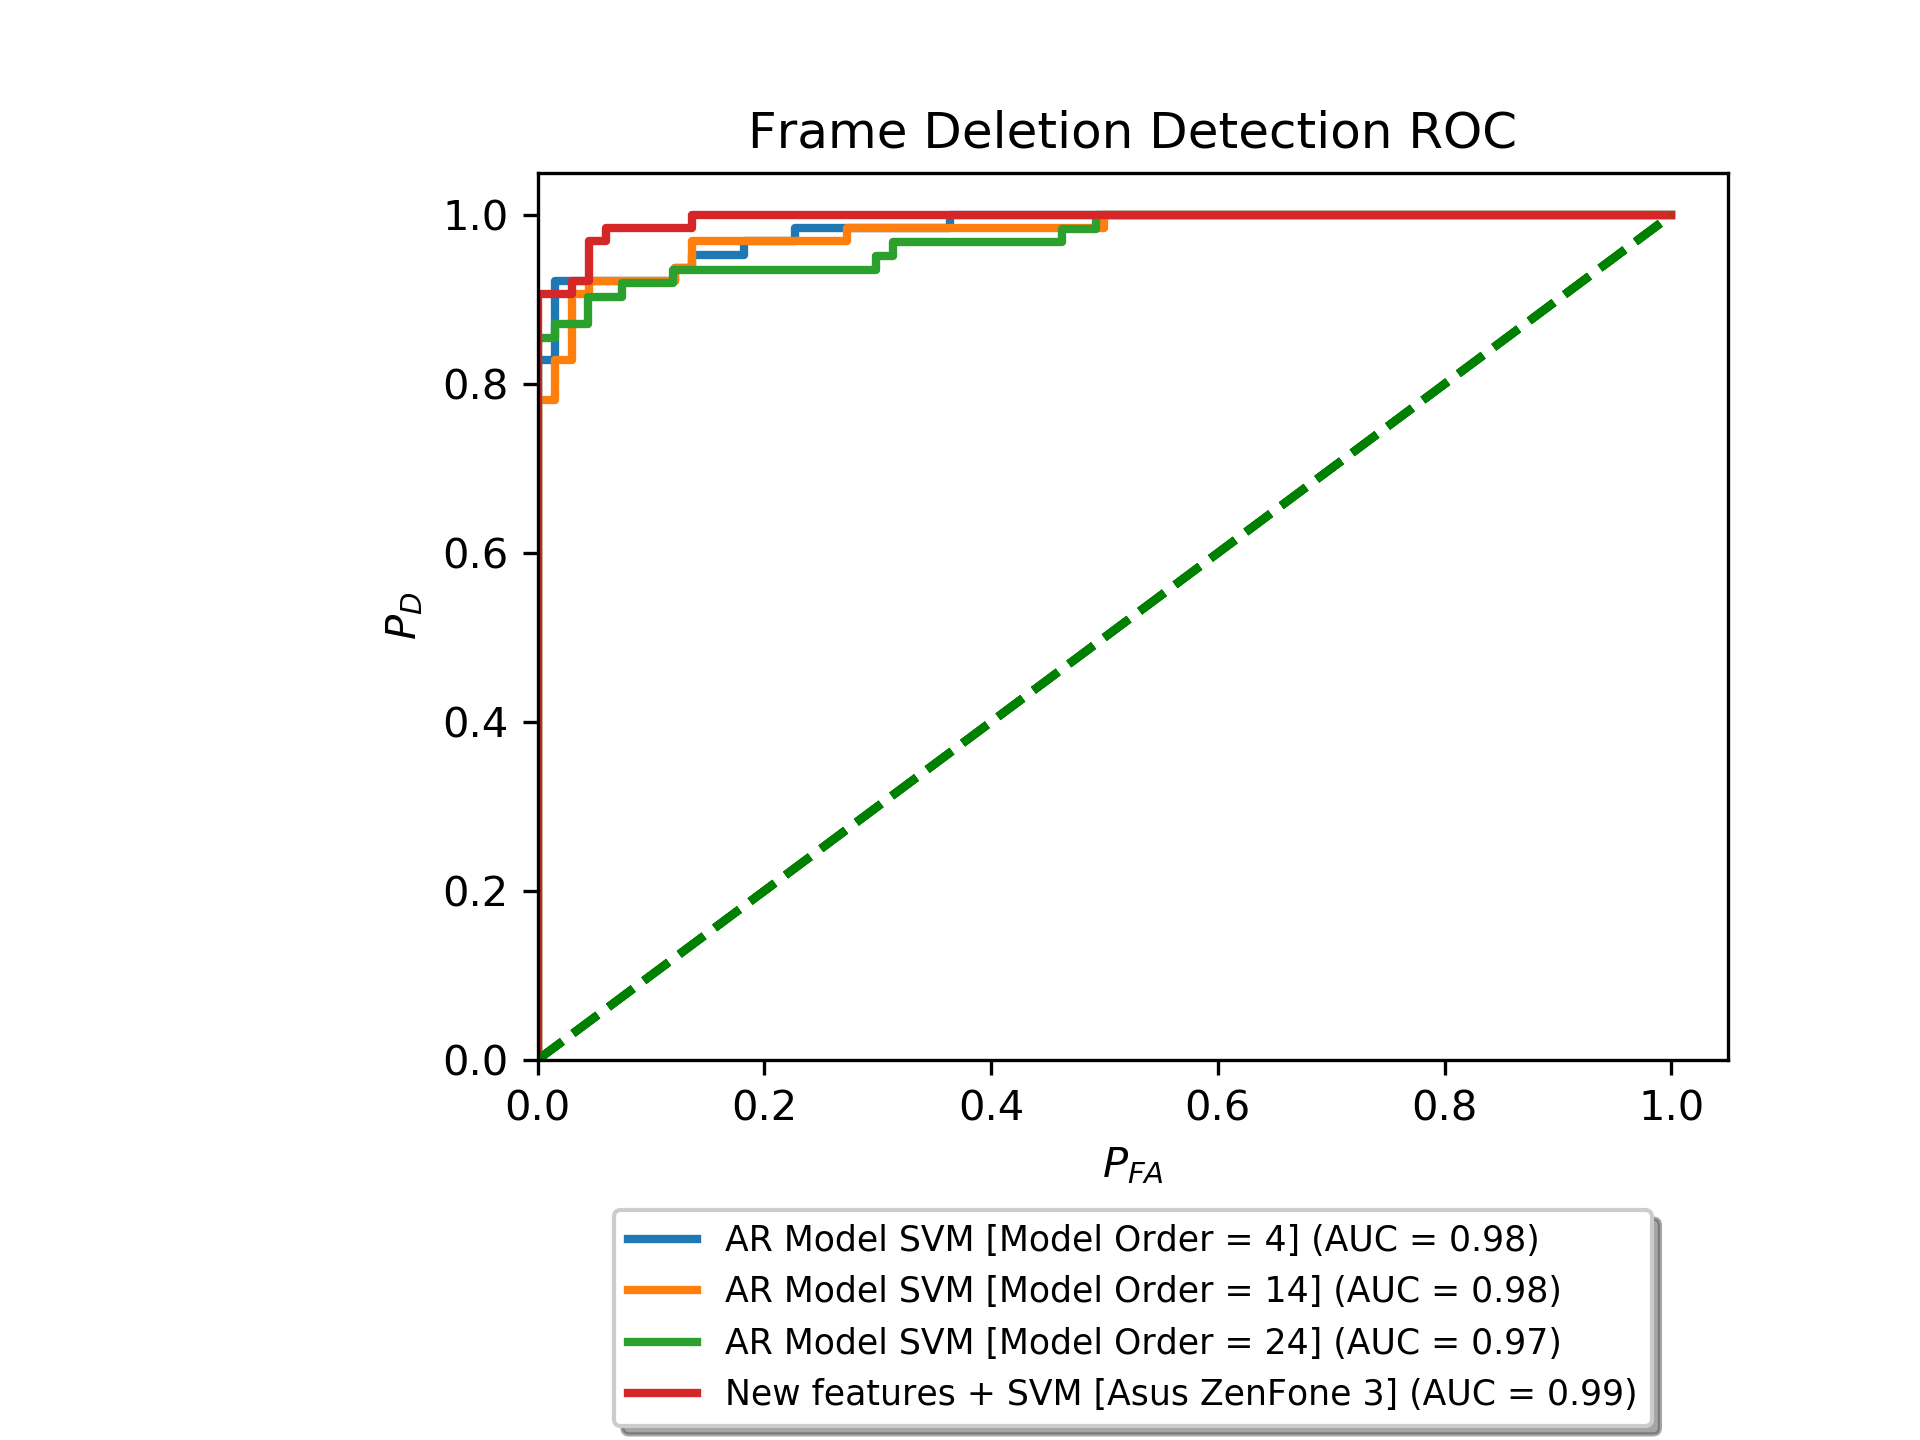
\includegraphics[width=0.9\linewidth]{../Graphs/perror_AR_model_comparison_roc.png}}
\caption{Graph of SVM ROC Curves for SVMs using traditional features versus an AR model for an ASUS Zen Fone 3}
\label{AR}
\end{figure}

\section{Problems I encountered}
\bi
\item The AR model features don't seem to produce a better classifier than the energy of $\hat{s}$, mean, variance, etc. features. As well, an increase in the model order of the AR model produces worse classification results. I would imagine this is likely due to over fitting on the AR model side of things. The maximum length of a video in any of the tests is around 200 frames long, and is not quite an order of magnitude larger than the number of model parameters. Though I am likely misinterpreting this. I am having a hard time understanding how these models are supposed to work.
\end{itemize}

\section{What I plan to do this week}
\bi
\item I plan on helping move the servers on Tuesday to the ECE server room.
\item I plan to continue testing the AR model and regular models on more data, as perhaps the AR model has less variance between phone models.
\item I plan to create more data to use for more complex experiments.
\item I plan to start writing the (throwaway) introduction to my thesis so that I can ground my future writings and set myself up for finishing. My completed draft is due by the end of week 8.
\end{itemize}


% Bib/refs go here if used

\begin{comment}
\pagebreak
%\bibliographystyle{plain}
\bibliographystyle{myIEEE}
\bibliography{StammRefs}
%\bibliography{StammRefs,kandasamy_v2,kandasamy}
\end{comment}


\end{document} 